

\section{Введение}
\subsection{Цель работы}
Лабораторная работа посвящена изучению способов повышения точности измерений путем их многократного повторения. Мы изучим методы статистической обработки данных, полученных в результате серии измерений одной и той же физической величины, и научимся оценивать погрешности, возникающие в процессе измерения. Исследование будет включать использование стандартного измерительного оборудования, математическое моделирование и анализ данных с использованием статистических методов.

\subsection{Решаемые задачи}
\begin{enumerate}
  \item Освоить методику использования измерительного прибора для
многократного прямого измерения физической величины.
  \item Выполнить простейшую статистическую обработку серии
результатов наблюдений при прямых измерениях.
\end{enumerate}

\section{Основная часть}

\subsection{Теоретическая часть}

\paragraph{Измерения}
Формула относительной погрешности прибора $\delta U$:
\begin{equation}
  \delta U = \pm (0,05 + 0,05  \frac{U_{\text{к}}}{U_{\text{х}}})\%
\end{equation}
где $U_{\text{к}}$ - конечное значение установленного предела измерений и $U_{\text{х}}$ - показания прибора. Для измерений на грубой шкале $U_{\text{к}}$ = 10 В, для измерений на точной шкале $U_{\text{к}}$ = 1 В.

Формула для нахождения среднего арифметического $\overline{U}$:
\begin{equation}
  \overline{U} = \frac{\sum_{i=1}^{n} U_i}{n}
\end{equation}
где $n$ - количество результатов отдельных наблюдений, $U_i$ - результат измерения отдельного наблюдения.

Вычисление погрешности прибора $\Delta U_{\text{приб}}$ определяется следующей формулой:
\begin{equation}
  \Delta U_{\text{приб}} = \frac{\delta U *\overline{U}}{100\%}
\end{equation}
Среднеквадратичное отклонение $\sigma$:
\begin{equation}
  \sigma \approx \sqrt{\frac{1}{n-1} \sum_{i = 1}^{n} (U_i -\overline{U}^2)}
\end{equation}
Средняя квадратичная погрешность среднего $\Delta U$:
\begin{equation}
  \Delta U = \sigma_{\overline{U}} \approx \frac{\sigma}{\sqrt{n}}
\end{equation}

\subsection{Эксперимент}
Вращая ручку потенциометра (делителя напряжения), были заданы диапазоны показаний шкалы прибора 0-10 В для грубой шкалы и 0-1 В для точной шкалы.
Задаваемое (по указанию преподавателя) напряжение многократно измерялось цифровым вольтметром. Все данные в ходе эксперимента записывались в протокол наблюдения.
\begin{figure}[ht!]
\centering
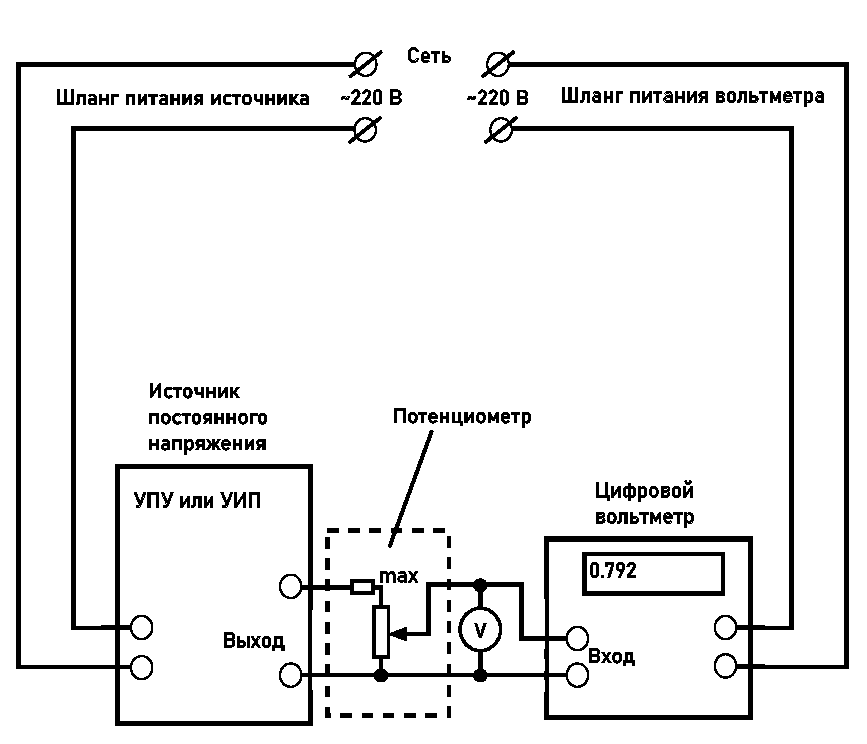
\includegraphics[width=0.8\textwidth]{схема.eps}
\caption{Схема установки}
\label{fig:sketch}
\end{figure}

\begin{figure}[ht!]
\centering
\includegraphics[width=0.8\textwidth]{Device}
\caption{Фотография установки}
\label{fig:device}
\end{figure}

\subsection{Обработка данных и обсуждение результатов}

\subsubsection{Исходный код}
Для написания программы, вычисляющей все требуемые данные, используется язык C++; среда разработки - Visual Studio.

Код программы разбит на несколько файлов: main.cpp, function.cpp, function.h. В файле function.h объявлены все используемые библиотеки и функции, которые реализует программа. Файл function.cpp определяет все функции программы, такие как: 
функция нахождения среднего арифметического, функция нахождения всех случайных отклонений из данной выборки, функция нахождения стандартных отклонений и т.д. Файл main.cpp отвечает за вывод вычисленных данных в файл с расширением .tex  в виде таблицы.

В этой функции (см. Листинг 1) реализовано считывание данных из файла. Возвращает данная функция результат в виде 0 (если мы успешно считали данные из файла) или 1 (если у нас не получилось считать данные). Эта функция также выполняет роль досрочного завершения программы в файле main.cpp.

\begin{lstlisting}[label=listing1, caption=Функция считывания данных из файла]
int readDataFromFile(const std::string& filename, std::vector<double>& values)
{
	std::ifstream file(filename);

	if (!file.is_open())
	{
		std::cerr << "File opening error!" << std::endl;
		return 1;
	}

	std::string line;
	while (getline(file, line))
	{
		if (line.empty())
		{
			continue;
		}

		values.push_back(std::stod(line));
	}

	file.close();

	return 0;
}

\end{lstlisting}

\begin{lstlisting}[label=listing2, caption=Реализация функции readDataFromFile()]
int main()
{
	std::vector<double> values;

	if (readDataFromFile("Accurate.csv", values) == 1)
	{
		return 1;
	}
    
...

    return 0
}
\end{lstlisting}

Функция sigma() дает значение среднего квадратичного отклонения $\sigma$:
\begin{verbatim}
double sigma(double sumStanDev, double n)
{
	return sqrt(sumStanDev / double(n - 1));
}
\end{verbatim}

Функция deltaU() дает значение средней квадратичной
погрешности среднего $\Delta U$:
\begin{verbatim}
double deltaU(double sigma, double n)
{
	return (sigma / sqrt(n));
}
\end{verbatim}

\subsubsection{Таблицы}

\begin{center}
\begin{table}[h!]
\centering
\caption{Результаты грубых измерений}
\label{tabl:1}
\begin{tabular}{|c|c|c|c|c|}
\hline
\begin{minipage}{7mm}
    № п.п. 
\end{minipage}&
\begin{minipage}{5cm}
    Диапазон показаний использованной шкалы прибора
\end{minipage} &
\begin{minipage}{5cm}
    Результаты отдельных наблюдений ($U_i$)
\end{minipage} &
\begin{minipage}{5cm}
    Погрешность прибора на данной шкале ($\Delta U_{\text{приб}}$)
\end{minipage}\\
\hline
{}&В&В&В\\
\hline
1 &	0-10  &	0.354 & 0.005169584 \\
2 &	0-10  &	0.354 & 0.005169584 \\
3 &	0-10  &	0.353 & 0.005183724 \\
4 &	0-10  &	0.354 & 0.005169584 \\
5 & 0-10  &	0.353 & 0.005183724 \\
6 & 0-10  &	0.353 & 0.005183724 \\
7 & 0-10  &	0.353 & 0.005183724 \\
8 & 0-10  &	0.353 & 0.005183724 \\
9 & 0-10  &	0.353 & 0.005183724 \\
10& 0-10  &	0.355 & 0.005155622 \\
\hline
\end{tabular}
\end{table}
\end{center}

\begin{center}
\begin{table}[h!]
\centering
\caption{Результаты точных измерений}
\label{tabl:2}
\begin{tabular}{|c|c|c|c|c|}
\hline
\begin{minipage}{7mm}
    № п.п. 
\end{minipage}&
\begin{minipage}{5cm}
    Результаты отдельных наблюдений ($U_i$)
\end{minipage} &
\begin{minipage}{5cm}
    Случайные отклонения от среднего $d_i = U_i - \overline{U}$
\end{minipage} &
\begin{minipage}{5cm}
    $d_i^2 = (U_i - \overline{U})^2$
\end{minipage}\\
\hline
{}&В&В&В$^2$\\
\hline
1 & 0.3589 & -0.000902 & 0.000000813604 \\
2 & 0.3598 & -0.000002 & 0.000000000004 \\
3 & 0.3620 & 0.002198 & 0.000004831204 \\
4 & 0.3566 & -0.003202 & 0.000010252804 \\
5 & 0.3613 & 0.001498 & 0.000002244004 \\
6 & 0.3576 & -0.002202 & 0.000004848804 \\
7 & 0.3585 & -0.001302 & 0.000001695204 \\
8 & 0.3581 & -0.001702 & 0.000002896804 \\
9 & 0.3582 & -0.001602 & 0.000002566404 \\
10 & 0.3579 & -0.001902 & 0.000003617604 \\
11 & 0.3601 & 0.000298 & 0.000000088804 \\
12 & 0.3576 & -0.002202 & 0.000004848804 \\
13 & 0.3577 & -0.002102 & 0.000004418404 \\
14 & 0.3574 & -0.002402 & 0.000005769604 \\
15 & 0.3620 & 0.002198 & 0.000004831204 \\


\hline
\end{tabular}
\end{table}
\end{center}

\begin{center}
\begin{table}[h!]
\centering
\caption{Результаты точных измерений}
\label{tabl:3}
\begin{tabular}{|c|c|c|c|c|}
\hline
\begin{minipage}{7mm}
    № п.п. 
\end{minipage}&
\begin{minipage}{5cm}
    Результаты отдельных наблюдений ($U_i$)
\end{minipage} &
\begin{minipage}{5cm}
    Случайные отклонения от среднего $d_i = U_i - \overline{U}$
\end{minipage} &
\begin{minipage}{5cm}
    $d_i^2 = (U_i - \overline{U})^2$
\end{minipage}\\
\hline
{}&В&В&В$^2$\\
\hline
16 & 0.3616 & 0.001798 & 0.000003232804 \\
17 & 0.3596 & -0.000202 & 0.000000040804 \\
18 & 0.3671 & 0.007298 & 0.000053260804 \\
19 & 0.3576 & -0.002202 & 0.000004848804 \\
20 & 0.3608 & 0.000998 & 0.000000996004 \\
21 & 0.3624 & 0.002598 & 0.000006749604 \\
22 & 0.3578 & -0.002002 & 0.000004008004 \\
23 & 0.3596 & -0.000202 & 0.000000040804 \\
24 & 0.3617 & 0.001898 & 0.000003602404 \\
25 & 0.3575 & -0.002302 & 0.000005299204 \\
26 & 0.3597 & -0.000102 & 0.000000010404 \\
27 & 0.3610 & 0.001198 & 0.000001435204 \\
28 & 0.3612 & 0.001398 & 0.000001954404 \\
29 & 0.3613 & 0.001498 & 0.000002244004 \\
30 & 0.3627 & 0.002898 & 0.000008398404 \\
31 & 0.3607 & 0.000898 & 0.000000806404 \\
32 & 0.3623 & 0.002498 & 0.000006240004 \\
33 & 0.3593 & -0.000502 & 0.000000252004 \\
34 & 0.3613 & 0.001498 & 0.000002244004 \\
35 & 0.3590 & -0.000802 & 0.000000643204 \\
36 & 0.3592 & -0.000602 & 0.000000362404 \\
37 & 0.3624 & 0.002598 & 0.000006749604 \\
38 & 0.3596 & -0.000202 & 0.000000040804 \\
39 & 0.3614 & 0.001598 & 0.000002553604 \\
40 & 0.3577 & -0.002102 & 0.000004418404 \\
41 & 0.3595 & -0.000302 & 0.000000091204 \\
42 & 0.3608 & 0.000998 & 0.000000996004 \\
43 & 0.3604 & 0.000598 & 0.000000357604 \\
44 & 0.3560 & -0.003802 & 0.000014455204 \\
45 & 0.3577 & -0.002102 & 0.000004418404 \\
46 & 0.3588 & -0.001002 & 0.000001004004 \\
47 & 0.3612 & 0.001398 & 0.000001954404 \\
48 & 0.3591 & -0.000702 & 0.000000492804 \\
49 & 0.3575 & -0.002302 & 0.000005299204 \\
50 & 0.3609 & 0.001098 & 0.000001205604 \\
\hline
\end{tabular}
\end{table}
\end{center}

\begin{center}
\begin{table}[h!]
\centering
\caption{Таблица для построения гистограммы и графика $\Delta n/n = f(x)$
}
\label{tabl:4}
\begin{tabular}{|c|c|c|c|c|}
\hline
\begin{minipage}{7mm}
    №
\end{minipage}&
\begin{minipage}{5cm}
    Границы интервалов (ширина интервала 0.001 В)
\end{minipage} &
\begin{minipage}{5cm}
    Число случаев ($\Delta$ n), когда результат наблюдения попадает в данный интервал
\end{minipage} &
\begin{minipage}{5cm}
    Доля полного числа результатов, попадающих в данный интервал ($\delta n = \frac{\Delta n}{n}$)
\end{minipage}\\
\hline
1 &	0.3560  &	2 & 0.04 \\
2 &	0.3570  &	11 & 0.22 \\
3 &	0.3580  &	5 & 0.1 \\
4 &	0.3590  &	10 & 0.2 \\
5 & 0.3600  &	6 & 0.12 \\
6 & 0.3610  &	9 & 0.18 \\
7 & 0.3620  &	6 & 0.12 \\
8 & 0.3630  &	0 & 0 \\
9 & 0.3640  &	0 & 0 \\
10& 0.3650  &	0 & 0 \\
11& 0.3660  &	0 & 0 \\
12& 0.3670  &	1 & 0.02 \\
\hline
\end{tabular}
\end{table}
\end{center}


\subsubsection{Графики}

\begin{figure}[ht!]
\centering
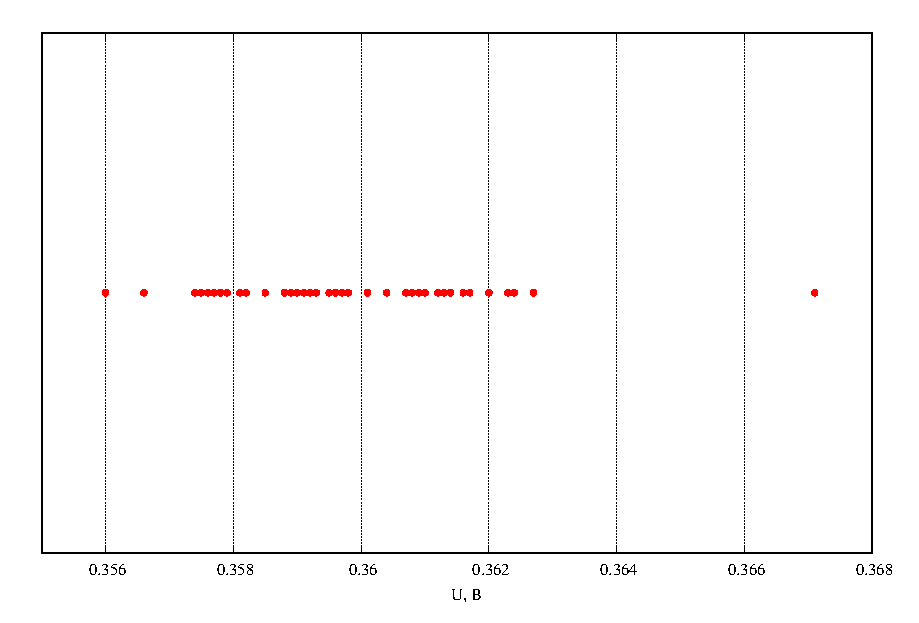
\includegraphics[width=0.8\textwidth]{voltage_i.eps}
\caption{Наблюдения на числовой оси}
\label{fig:plot1}
\end{figure}
$U_{min} = 0.3560$ В, $U_{max} = 0.3671$ В.
\begin{figure}[ht!]
\centering
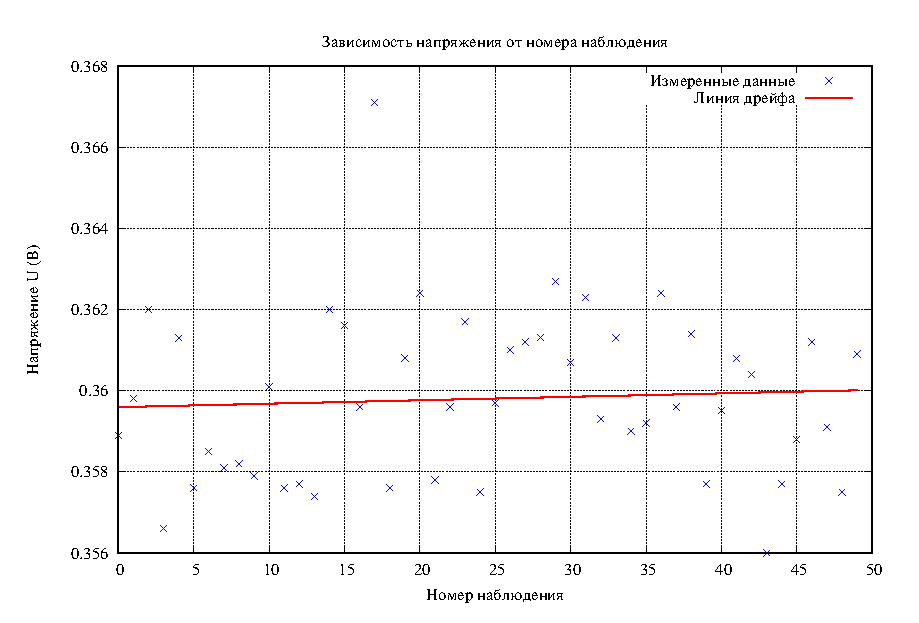
\includegraphics[width=0.8\textwidth]{voltage_drift.eps}
\caption{Зависимость результатов наблюдений от времени}
\label{fig:plot}
\end{figure}

\begin{figure}[ht!]
\centering
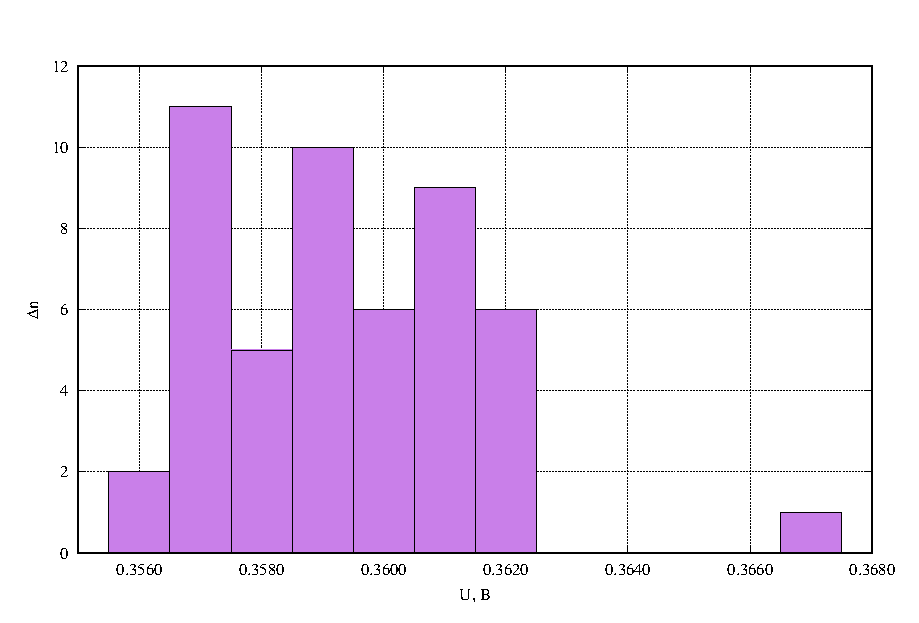
\includegraphics[width=0.8\textwidth]{histogramma.eps}
\caption{Гистограмма}
\label{fig:plot2}
\end{figure}

\begin{figure}[ht!]
\centering
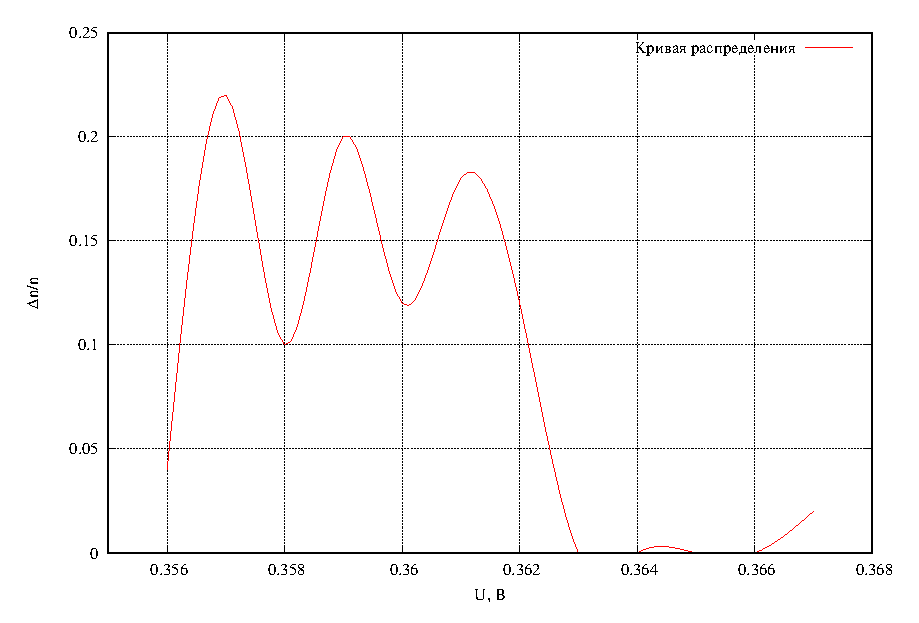
\includegraphics[width=0.8\textwidth]{delta_n_vs_voltage.eps}
\caption{График распределения}
\label{fig:plot3}
\end{figure}

Благодаря графику распределения можно получить приблизительную оценку для среднего квадратичного отклонения $\sigma \approx 0.002$. 

Используя формулу (4), получаем, что $\sigma \approx 0.002043$.

Дисперсия: $\sigma^2 \approx 0.000004$ В$^2$.

Определим среднюю квадратичную погрешность среднего по формуле (5): $\Delta U \approx 0.000289$ В.


Предел допускаемой погрешности прибора на точной шкале $\omega = 0.000679$, вычисленный по формуле (3). Можно  заключить, что $\omega$ и $\Delta U$ величины одного порядка ($\frac{\omega}{4} < \Delta U < 4\omega$).

Результат: $U = \overline{U}  + \Delta U= 0.359802 \pm 0.000289$ В.

\section{Вывод}
В ходе выполнения работы я приобрел практические навыки использования измерительных приборов для многократных прямых измерений физических величин. В частности, я научился работать с цифровым вольтметром для измерения напряжения и освоил методы статистической обработки результатов, включая расчет дисперсии и среднеквадратичного отклонения. Также приобрел навык работы с такими программами, как gnuplot для реализации графиков и inkscape для создания блок-схемы установки. 
% Список литературы
% Для отчёта он не обязателен
\begin{thebibliography}{9}

%ссылка на репозиторий с исходныим кодом отчета и всех расчетных программ обязательна 
\bibitem{repo}
\url{https://github.com/st117210/Workshop1.git}  

\end{thebibliography}
\clearpage
\appendix